\chapter{Implementasi dan Pengujian}

\section{Implementasi}
Berdasarkan hasil analisis serta perancangan yang dituliskan pada Bab III, dilakukan implementasi ILE pada platform web KodeBareng. Dalam bab ini dijelaskan mengenai implementasi dan pengujian terhadap ILE yang dibuat.

\subsection{Batasan Implementasi}
Implementasi dilakukan menggunakan teknologi yang telah dipakai pada KodeBareng sebelumnya. Daftar teknologi dan \textit{framework} yang digunakan pada KodeBareng dapat dilihat pada \autoref{tab:tech-stack}.

\begin{longtable}[c]{|>{\setlength{\baselineskip}{0.75\baselineskip}}p{0.3\linewidth}|>{\setlength{\baselineskip}{0.75\baselineskip}}p{0.4\linewidth}|}
  \caption{\textit{Tech stack} yang digunakan oleh KodeBareng}
  \label{tab:tech-stack}                                                                                            \\
  \hline
  \rowcolor{gray!30}
  \textbf{Nama Sistem}                                     & \textbf{Teknologi / \textit{Framework} yang digunakan} \\ \hline
  \endfirsthead
  %
  \endhead
  %
  \textit{Frontend}                                        & NuxtJS, Cloudflare Pages                               \\ \hline
  \textit{Backend}                                         & ExpressJS, Linux, NodeJS, Docker                       \\ \hline
  CMS (\textit{Content Management System})                 & NextJS, Netlify                                        \\ \hline
  \textit{Autograder} (sekarang menjadi \textit{Executor}) & ExpressJS, Linux, NodeJS, Docker, Python 3.9           \\ \hline
\end{longtable}

Selain dari teknologi yang digunakan, terdapat juga batasan dari bahasa pemrograman yang dapat divisualisasikan eksekusinya yaitu Python sesuai dengan kelas pembelajaran pemrograman yang sudah ada pada platform web KodeBareng.

% Please add the following required packages to your document preamble:
% \usepackage{longtable}
% Note: It may be necessary to compile the document several times to get a multi-page table to line up properly
\footnotesize
\begin{longtable}[c]{|l|l|}
  \caption{Cakupan implementasi ILE}
  \label{tab:ile-scope}                                                              \\
  \hline
  \rowcolor{gray!30}
  \normalsize\textbf{Concepts}                  & \normalsize Termasuk Implementasi? \\ \hline
  \endhead
  %
  \textbf{Input/Output}                         &                                    \\ \hline
  Standard Input/Output                         & Termasuk                           \\ \hline
  File I/O                                      & Tidak Termasuk                     \\ \hline
  \textbf{Variables}                            &                                    \\ \hline
  Variable types                                & Termasuk                           \\ \hline
  Variable scope                                & Termasuk                           \\ \hline
  Assignment of values to variables             & Termasuk                           \\ \hline
  \textbf{Selection and repetition structures}  &                                    \\ \hline
  If statement                                  & Termasuk                           \\ \hline
  While loop                                    & Termasuk                           \\ \hline
  For loop                                      & Termasuk                           \\ \hline
  \textbf{Methods}                              &                                    \\ \hline
  Method structure                              & Termasuk                           \\ \hline
  Method frames                                 & Termasuk                           \\ \hline
  Message passing                               & Termasuk                           \\ \hline
  Return values                                 & Termasuk                           \\ \hline
  Recursion                                     & Termasuk                           \\ \hline
  Lambda function                               & Tidak Termasuk                     \\ \hline
  \textbf{Arrays}                               &                                    \\ \hline
  Arrays as objects                             & Termasuk                           \\ \hline
  Array structure                               & Termasuk                           \\ \hline
  Arrays of primitives                          & Termasuk                           \\ \hline
  Arrays of references                          & Tidak Termasuk                     \\ \hline
  Array index                                   & Termasuk                           \\ \hline
  List Comprehension                            & Tidak Termasuk                     \\ \hline
  \textbf{Algorithms}                           &                                    \\ \hline
  Search algorithms                             & Tidak Termasuk                     \\ \hline
  Sort algorithms                               & Tidak Termasuk                     \\ \hline
  Data structures (linked list and binary tree) & Tidak Termasuk                     \\ \hline
  \textbf{Additional requirements}              &                                    \\ \hline
  Debugging                                     & Tidak Termasuk                     \\ \hline
  Standard libraries                            & Termasuk                           \\ \hline
\end{longtable}
\normalsize

\subsection{Implementasi Sistem Eksekutor}
[\hl{TODO: MASUKIN INPUT, PROSES, OUTPUT MASING2 KOMPONEN}]
[\hl{TODO: MASUKIN KOMPONEN/LIBRARY YANG DIGUNAKNA UNTUK TIAP KOMPONEN}]
[\hl{TODO: MASUKIN TREE VIEW TIAP KOMPONEN LETAKNYA ADA DIMANA AJA}]
[\hl{TODO: MASUKIN HAMBATAN DAN SOLUSI DI TIAP KOMPONEN}]

Sistem Eksekutor menggunakan \textit{tech stack} berupa ExpressJS dengan Typescript yang dijalankan pada NodeJS menggunakan kakas \textit{nodemon}. Sistem tersebut kemudian diisolasi menggunakan Docker dengan \textit{image} Debian 10 dan dilakukan instalasi Python 3.9. Terdapat juga kakas berupa \textit{swagger} yang digunakan untuk dokumentasi rute-rute yang terdapat pada sistem ini.

\subsubsection{Modifikasi Komponen Controller}
Pada sistem ini sudah terdapat \textit{controller} pada tiap bagian rute untuk mengolah data yang diberikan. Pada Tugas Akhir ini, ditambahkan rute untuk melakukan visualisasi serta \textit{controller} untuk mengolah data tersebut. \textit{Controller} mendapatkan masukan berupa kode program berupa \textit{string} serta input berupa \verb|array of string| untuk diberikan pada program yang dieksekusi. Kemudian, \textit{Controller} melakukan pengecekan apakah kode diperbolehkan untuk dieksekusi, lalu menuliskan kode pada file Python sementara. Setelah itu, \textit{controller} menjalankan \textit{helper} berupa Komponen Executor dan Parser dengan memberikan masukan berupa lokasi \textit{file} kode program serta \textit{input} yang akan diberikan pada program.

  [\hl{TODO: MASUKIN CONTOH HASIL INPUT CONTROLLER UNTUK KOMPONEN EXECUTOR DAN PARSER}]

\subsubsection{Implementasi Komponen Executor}
Komponen Executor merupakan komponen yang digunakan untuk mengeksekusi kode program menggunakan PDB. Komponen ini membutuhkan masukan berupa lokasi \textit{file} berisi kode program yang akan dieksekusi serta \textit{input} yang akan diberikan kepada program. Terdapat 3 tahapan utama dalam komponen ini, yaitu tahap inisialisasi, tahap pengecekan, serta tahap pengumpulan data.

Tahap inisialisasi adalah tahap menginjeksi kode tambahan ke dalam eksekusi Python untuk keperluan Komponen Executor dan Parser. Pada tahap ini, dimasukkan kode untuk mengubah keluaran Python menjadi JSON agar dapat diolah oleh NodeJS. Selain itu, terdapat juga fungsi-fungsi tambahan untuk mendapatkan tipe data pada Python serta melakukan \textit{deep iteration} untuk mendapatkan informasi tipe data serta id dari variabel yang bertipe \textit{sequence} atau \textit{hashmap}. Tahap inisialisasi hanya dilakukan sekali untuk setiap kode program yang dijalankan.

Setelah inisialisasi dijalankan, dilakukan tahap pengecekan yaitu untuk mengecek apakah eksekusi program sedang berada di luar kode program yang seharusnya karena terkadang PDB menjalankan kode program pada modul \textit{standard library} (\textit{built-in module}). Apabila program sedang mengeksekusi baris diluar kode program (penentuan dilakukan oleh Komponen Parser), maka Komponen Executor akan mengeksekusi perintah untuk kembali keluar modul tersebut dan kembali pada kode program awal. Setelah itu, Komponen Executor akan melanjutkan langkah eksekusi tanpa melalui tahapan pengumpulan data.

Apabila program lolos dari tahap pengecekan (program tidak berada di luar kode program), maka dilakukan tahap pengumpulan data. Tahap pengumpulan data adalah tahap pengumpulan \textit{fields} yang berada pada \textit{runtime memory} seperti variabel, fungsi dan metode, serta modul yang telah dimuat. Tahap ini terbagi menjadi 3 subtahap, yaitu tahap \verb|Local|, \verb|Global|, dan \verb|Stack|. Subtahap \verb|Lokal| adalah subtahap mengeksekusi perintah untuk mengumpulkan \textit{fields} pada memori lokal suatu \textit{stack frame}. Subtahap \verb|Global| adalah subtahap mengeksekusi perintah untuk mengumpulkan \textit{fields} pada memori global suatu program. Subtahap \verb|Stack| adalah subtahap mengeksekusi perintah untuk mengumpulkan data pada \textit{stack frame} berupa baris kode yang sedang dieksekusi, \textit{return value}, serta daftar \textit{frame} yang tersimpan pada \textit{stack frame}.Hasil keluaran dari seluruh perintah tersebut akan diolah oleh Komponen Parser.

Setelah Komponen Executor dan Parser melewati tahap pengumpulan data dan tidak terjadi error, maka Komponen Executor akan melanjutkan langkah eksekusi kode sekaligus perintah yang digunakan untuk pengecekan \textit{error}, serta me-\textit{reset} data-data dan tahapan-tahapan yang dilakukan lalu kembali pada tahap pengecekan. Apabila terdapat error selama tahap pengumpulan data, maka Komponen Executor akan mematikan program yang sedang dieksekusi. Apabila jumlah langkah atau lama waktu eksekusi sudah melebihi batas yang telah ditentukan, maka Komponen Executor juga akan mematikan program yang sedang dieksekusi.

  [\hl{TODO: MASUKIN CONTOH HASIL KELUARAN KOMPONEN EXECUTOR }]

\subsubsection{Implementasi Komponen Parser}
Komponen Parser merupakan komponen yang digunakan untuk mengolah hasil keluaran Komponen Executor. Komponen ini juga menentukan logika dan langkah yang akan diambil oleh Komponen Executor. Komponen ini membutuhkan masukan berupa \verb|array of string| yang merupakan hasil keluaran Komponen Executor yang telah dipisahkan tiap barisnya. Terdapat 2 tahapan utama dalam komponen ini, yaitu tahap pengecekan dan tahap pengumpulan data.

Tahap pengecekan dilakukan bersamaan dengan Komponen Executor melakukan tahap pengecekan. Pada tahap ini, terdapat beberapa subtahap yaitu pengecekan \textit{input}, pengecekan \textit{output}, serta pengecekan eksekusi \textit{built-in module}.

Pada subtahap pengecekan \textit{input}, dilakukan pengecekan terhadap \textit{signature output} dari PDB serta pengecekan waktu eksekusi suatu baris. Apabila tidak ditemukan \textit{signature output} dari PDB atau waktu eksekusi suatu baris melebihi batas, maka komponen ini akan memasukkan \textit{input} (melalui Komponen Executor) sesuai dengan \textit{input} yang dberikan oleh \textit{controller}. Apabila tidak ada \textit{input} yang diberikan oleh \textit{controller} atau \textit{input} yang diberikan oleh \textit{controller} kurang dari jumlah input yang dibutuhkan, maka Komponen Parser akan memasukkan \textit{event} untuk meminta tambahan input dan mematikan program yang dieksekusi.

Setelah itu, dilakukan subtahap pengecekan \textit{output} untuk mengecek dan mengolah apabila program mengeluarkan \textit{output} atau \textit{error} setelah melanjutkan langkah eksekusi. Apabila program mengeluarkan \textit{error}, maka Komponen Parser akan mengolah \textit{error} dan \textit{traceback} yang dikeluarkan dan menyimpannya ke dalam \textit{event} lalu mematikan program. Apabila program mengeluarkan \textit{output}, maka Komponen Parser akan mengolah \textit{output} tersebut dan memasukkannya ke dalam daftar \textit{output} program.

Kemudian, dilakukan subtahap pengecekan eksekusi \textit{built-in module} yang telah dijelaskan pada Komponen Executor sebelumnya. Komponen Parser akan mengecek hasil keluaran dari perintah yang dimasukkan oleh Komponen Executor, kemudian apabila terdeteksi \textit{error} maka Komponen Parser tidak akan mengolah data hingga Komponen Executor melanjutkan langkah eksekusi program.

Setelah seluruh tahapan dalam tahap pengecekan selesai, Komponen Parser akan memasuki tahap pengumpulan data yang tahapannya sama dengan tahapan pengumpulan data yang terdapat pada Komponen Executor. Hasil keluaran Komponen Executor diolah dengan mengolah keluaran JSON. Apabila keluaran tersebut tidak dapat diolah sebagai JSON, maka Komponen Parser akan menghasilkan \textit{error}, disimpan sebagai \textit{event} lalu mematikan program. Setelah semua subtahap pengumpulan data dilakukan, Komponen Parser akan mengolah seluruh hasil pengumpulan data ke dalam daftar \verb|ExecutionResult| yang akan dikembalikan kepada \textit{controller} saat program telah selesai atau dimatikan dan menjadi hasil yang dapat divisualisasikan pada Sistem Frontend.

  [\hl{TODO: MASUKKAN CONTOH HASIL KELUARAN KOMPONEN PARSER}]

\subsection{Implementasi Backend}
\subsubsection{Implementasi Komponen Helper}
Komponen Helper merupakan komponen yang digunakan untuk mendeteksi perintah-perintah yang tidak diperbolehkan eksekusi pada kode. Apabila tidak terdapat perintah yang dilarang pada kode, maka kode diteruskan kepada sistem Executor dan mengembalikan hasilnya. Apabila terdapat perintah yang dilarang pada kode, maka kode akan ditolak dan tidak akan dieksekusi.


\subsection{Implementasi Frontend}

\subsubsection{Implementasi Komponen Web IDE}
Komponen Web IDE dibuat menggunakan Monaco Editor yang dibuat oleh Microsoft. Komponen ini dapat memperlihatkan \textit{syntax highlighting} pada kode, menunjukkan angka baris, serta navigasi menggunakan \textit{scrollbar} yang memiliki \textit{overview} dari seluruh kode program.

\subsubsection{Implementasi Komponen Visualizer}
Komponen Visualizer merupakan komponen yang dapat memvisualisasikan hasil olahan \textit{stack trace} suatu kode. Komponen ini dapat berinteraksi dengan Web IDE untuk menunjukkan lokasi eksekusi suatu langkah dengan memberikan warna pada baris eksekusi, serta membuat tabel data pada memori pada setiap \textit{stack frame}. Pengguna dapat mengubah alur maju mundur visualisasi, melihat isi data dan baris kode yang sedang dieksekusi pada setiap \textit{stack frame}, serta melihat perubahan pada data dalam memori.


\section{Pengujian}

\subsection{Tujuan Pengujian}
Tujuan dari pengujian ini adalah untuk mendapatkan data terkait dampak ILE yang telah dibuat terhadap pemahaman pelajar mengenai konsep serta alur kerja eksekusi kode program.

\subsection{Lingkungan Pengujian}
Pengujian  dilakukan terhadap faktor pemahaman siswa mengenai konsep pemrograman serta alur kerja eksekusi kode program. Maka dari itu, pengujian dilakukan berdasarkan pengujian pada \textcite{mayer1981psychology} untuk faktor pemahaman konsep program serta pada \textcite{moons2013pilot} untuk faktor pemahaman alur kerja serta.

  [\hl{TODO: MASUKIN MATERI YANG DDIPAKAI, DEMOGRAFIS, SPEK HARDWARE SERVER}]

\begin{figure}[H]
  \centering
  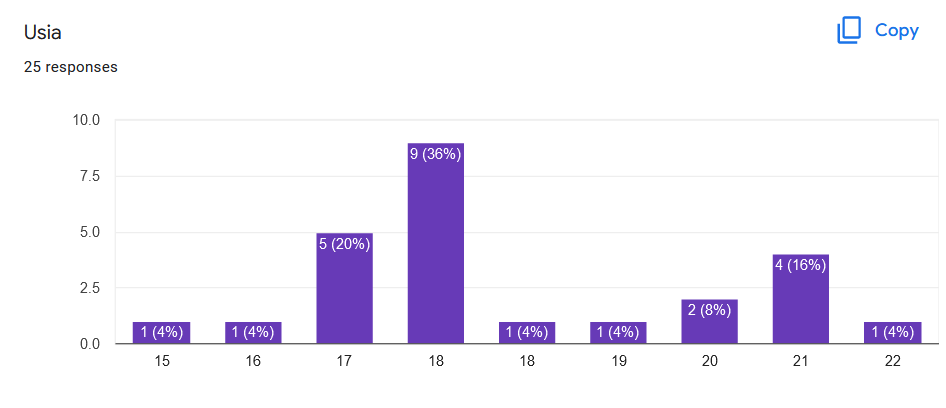
\includegraphics[width=0.7\textwidth]{chapter4/demografis-usia.png}
  \caption{Demografis usia peserta eksperimen} \label{fig:demografis-usia}
\end{figure}
\begin{figure}[H]
  \centering
  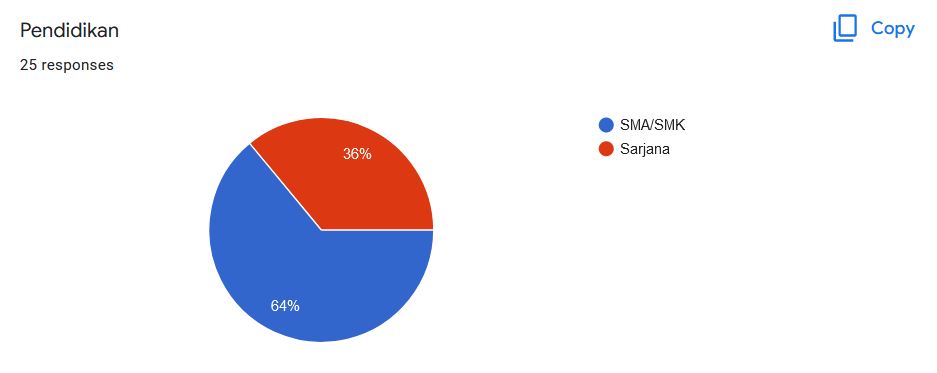
\includegraphics[width=0.7\textwidth]{chapter4/demografis-pendidikan.png}
  \caption{Demografis tahap pendidikan peserta eksperimen} \label{fig:demografis-pendidikan}
\end{figure}
\begin{figure}[H]
  \centering
  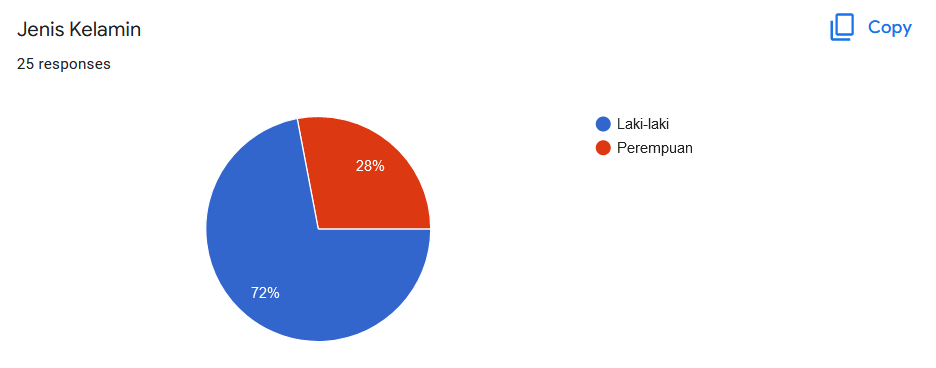
\includegraphics[width=0.7\textwidth]{chapter4/demografis-kelamin.png}
  \caption{Demografis jenis kelamin peserta eksperimen} \label{fig:demografis-kelamin}
\end{figure}

\subsection{Skenario dan Hasil Pengujian}
[\hl{TODO: MASUKIN TABEL ACC TESTING, MASUKIN CONTROL EXPERIMENT}]

Pengujian dilakukan pada platform web KodeBareng dengan menggunakan kelas pembelajaran khusus untuk melakukan pengujian. Pengujian dilakukan pada 2 grup dengan masing-masing grup memiliki 10 orang penguji, yaitu grup kontrol dan grup perlakuan. Grup kontrol mendapatkan materi pembelajaran tanpa adanya integrasi visualisasi eksekusi kode, sementara grup perlakuan mendapatkan materi pembelajaran yang terdapat integrasi visualisasi eksekusi kode. Setiap grup mendapatkan materi pembelajaran yang sama serta kuesioner setelah melakukan pembelajaran.

Kuesioner memiliki 2 bagian pertanyaan, masing-masing untuk tiap faktor yang diuji. Bagian pertama berdasar pada \textcite{mayer1981psychology} yang terdapat suatu kode untuk kemudian diminta kepada penguji untuk dijelaskan konsep-konsepnya di dalam kode tersebut. Bagian kedua berdasar pada \textcite{moons2013pilot} juga terdapat suatu kode yang telah diperumit penamaannya dan diminta kepada penguji untuk menjelaskan alur kerja program tersebut. Pada bagian kedua, penguji pada grup perlakuan dapat melakukan visualisasi eksekusi pada kode tersebut, sementara pada grup kontrol tidak.


\section{Analisis Hasil Pengujian}
 [\hl{TODO: MASUKIN HASIL OLAHAN DATA NUMERIK, DATA LOGGING, SAMA DATA KUESIONER}]

\subsection{Analisis Data Kuesioner}
\begin{figure}[H]
  \centering
  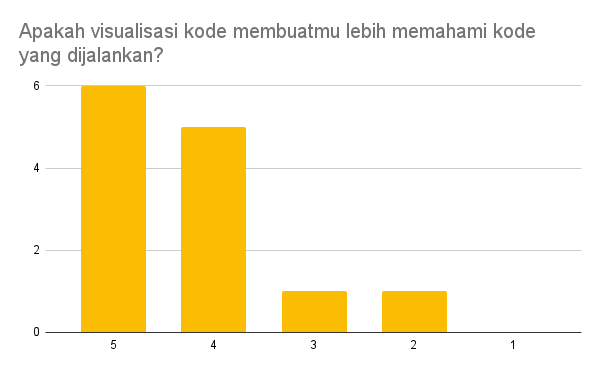
\includegraphics[width=0.7\textwidth]{chapter4/kuesioner-memahami.png}
  \caption{Apakah ILE membantu memahami kode?} \label{fig:kuesioner-memahami}
\end{figure}
\blindtext

\begin{figure}[H]
  \centering
  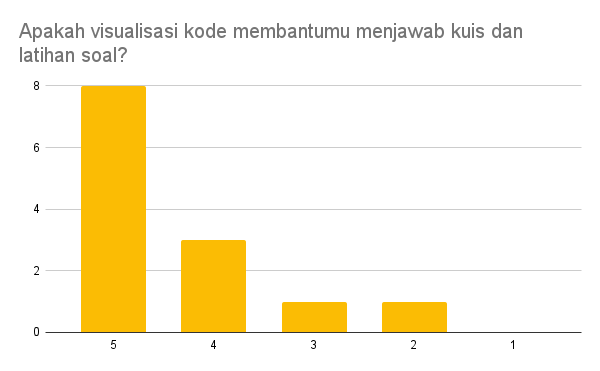
\includegraphics[width=0.7\textwidth]{chapter4/kuesioner-soal.png}
  \caption{Apakah ILE membantu menjawab latihan soal?} \label{fig:kuesioner-soal}
\end{figure}
\blindtext

\begin{figure}[H]
  \centering
  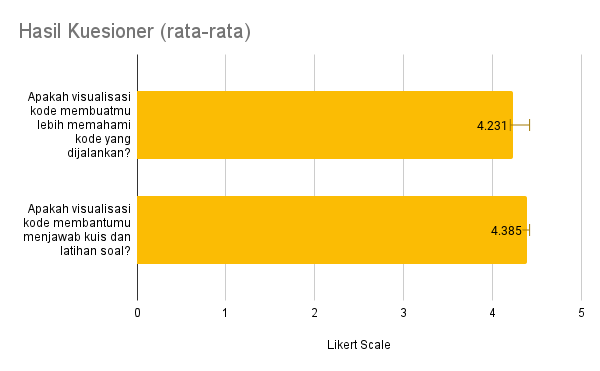
\includegraphics[width=0.9\textwidth]{chapter4/kuesioner-average.png}
  \caption{Hasil kuesioner ILE} \label{fig:kuesioner-average}
\end{figure}
\blindtext

\subsection{Analisis Data Eksperimen}
\begin{figure}[H]
  \centering
  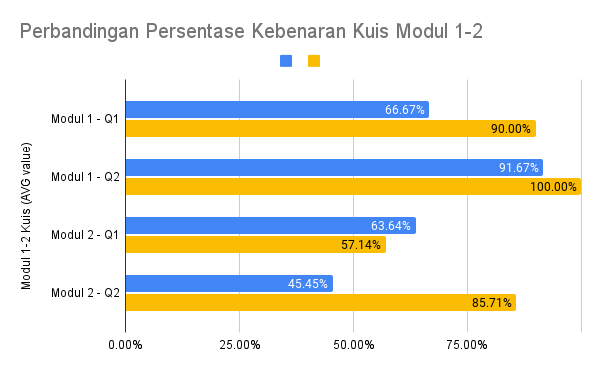
\includegraphics[width=0.9\textwidth]{chapter4/eksperimen-k1k2-kebenaran-all.png}
  \caption{Hasil eksperimen modul 1-2 soal kuis} \label{fig:eksperimen-k1k2-kebenaran-all}
\end{figure}
\begin{figure}[H]
  \centering
  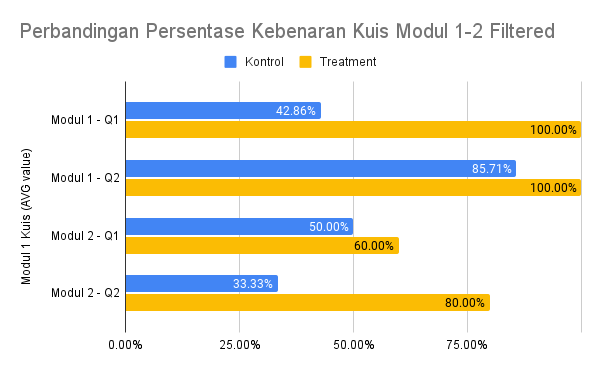
\includegraphics[width=0.9\textwidth]{chapter4/eksperimen-k1k2-kebenaran-awam.png}
  \caption{Hasil eksperimen modul 1-2 soal kuis khusus yang masih awam} \label{fig:eksperimen-k1k2-kebenaran-awam}
\end{figure}
\blindtext
\begin{figure}[H]
  \centering
  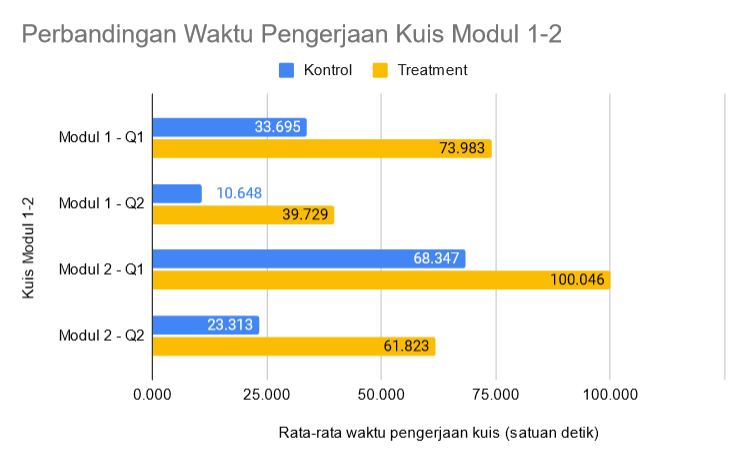
\includegraphics[width=0.9\textwidth]{chapter4/eksperimen-k1k2-waktu.png}
  \caption{Waktu menjawab soal kuis modul 1-2} \label{fig:eksperimen-k1k2-waktu}
\end{figure}
\blindtext

\begin{figure}[H]
  \centering
  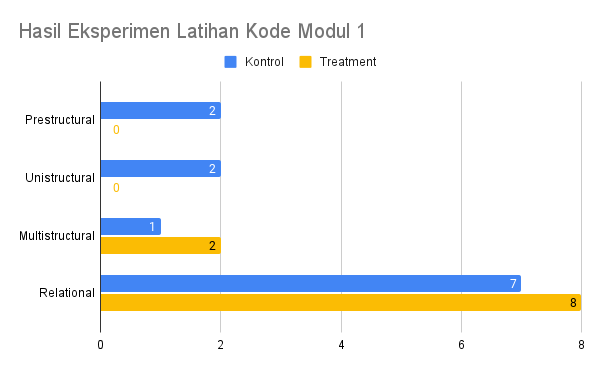
\includegraphics[width=0.9\textwidth]{chapter4/eksperimen-lk1-all.png}
  \caption{Hasil eksperimen modul 1 soal latihan kode} \label{fig:eksperimen-lk1-all}
\end{figure}
\begin{figure}[H]
  \centering
  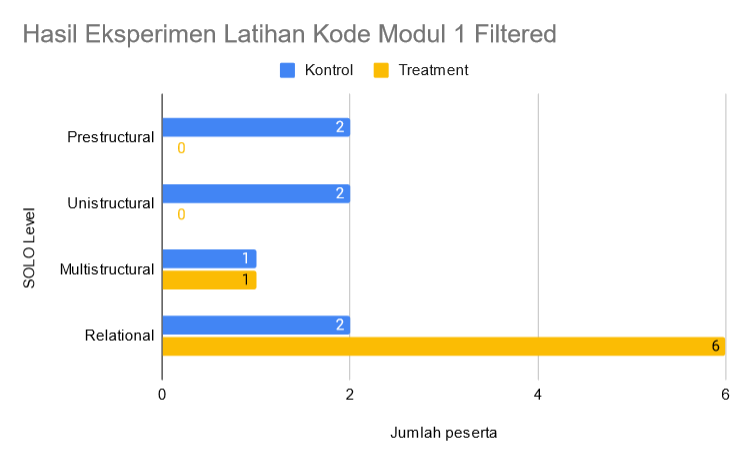
\includegraphics[width=0.9\textwidth]{chapter4/eksperimen-lk1-awam.png}
  \caption{Hasil eksperimen modul 1 soal latihan kode khusus yang masih awam} \label{fig:eksperimen-lk1-awam}
\end{figure}
\blindtext
\begin{figure}[H]
  \centering
  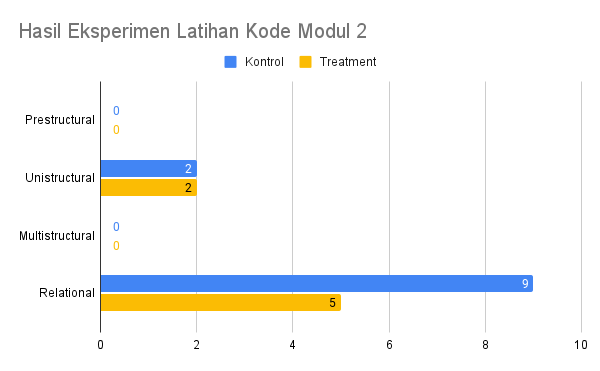
\includegraphics[width=0.9\textwidth]{chapter4/eksperimen-lk2-all.png}
  \caption{Hasil eksperimen modul 2 soal latihan kode} \label{fig:eksperimen-lk2-all}
\end{figure}
\begin{figure}[H]
  \centering
  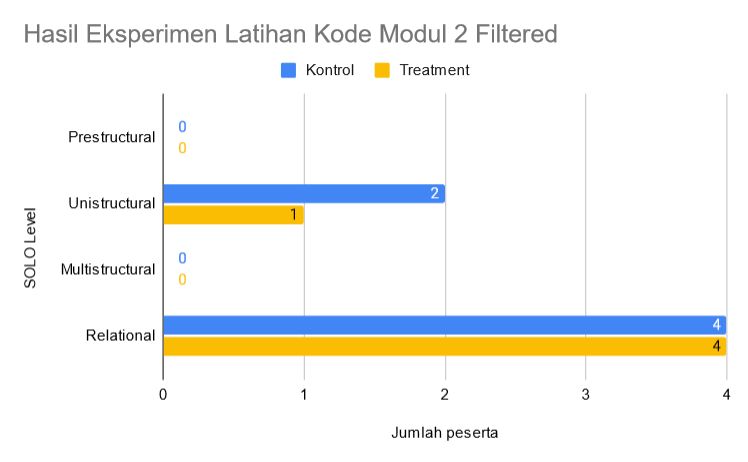
\includegraphics[width=0.9\textwidth]{chapter4/eksperimen-lk2-awam.png}
  \caption{Hasil eksperimen modul 2 soal latihan kode khusus yang masih awam} \label{fig:eksperimen-lk2-awam}
\end{figure}
\blindtext

\begin{figure}[H]
  \centering
  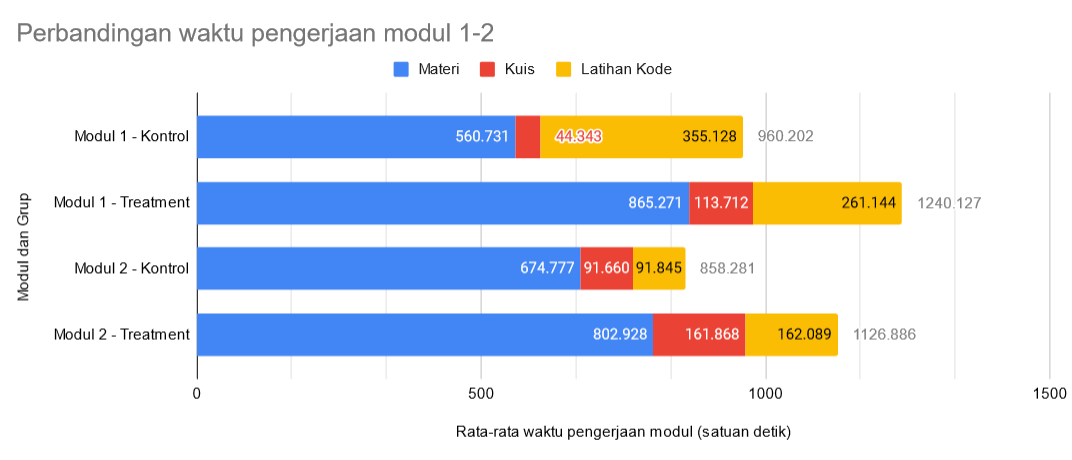
\includegraphics[width=0.9\textwidth]{chapter4/eksperimen-m1m2-waktu.png}
  \caption{Perbandingan waktu pengerjaan modul 1 dan modul 2} \label{fig:eksperimen-m1m2-waktu}
\end{figure}
\blindtext

\subsection{Ancaman Kebenaran}
\blindtext